\section{Kadek Diva Krishna Murti (1174006)}
\subsection{Instalasi Map Server}
\begin{enumerate}
	\item  Download installer Map Server di \href{https://ms4w.com/}{https://ms4w.com/}. Pilih yang .exe.
	\hfill\break
	\begin{figure}[H]
		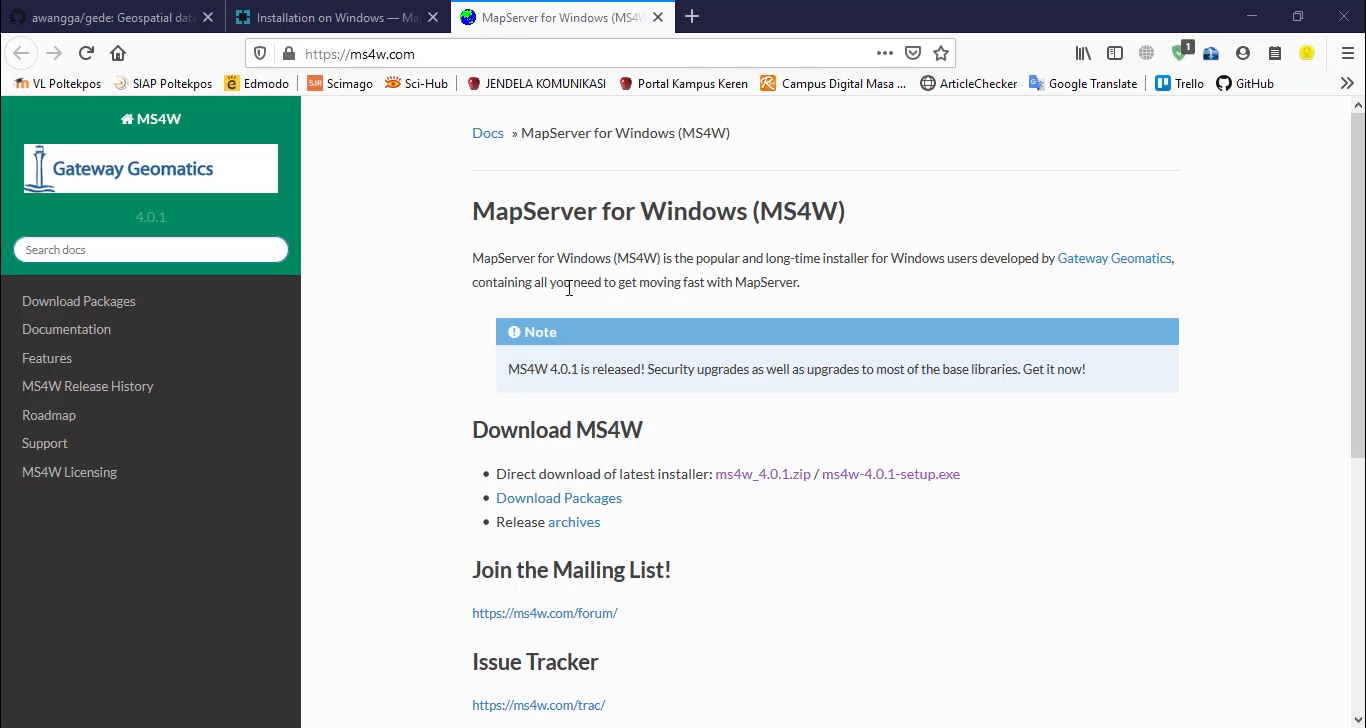
\includegraphics[width=8cm]{figures/1174006/4/1.png}
		\centering
		\caption{Download installer Map Server.}
	\end{figure}
	\item  Setelah selesai di download, klik dua kali pada installer.
	\hfill\break
	\begin{figure}[H]
		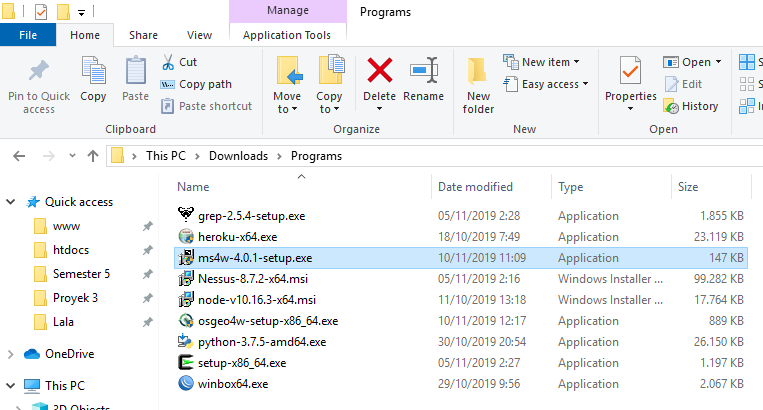
\includegraphics[width=8cm]{figures/1174006/4/2.png}
		\centering
		\caption{Klik dua kali pada installer.}
	\end{figure}
	\item  Kemudian klik "I Agree".
	\hfill\break
	\begin{figure}[H]
		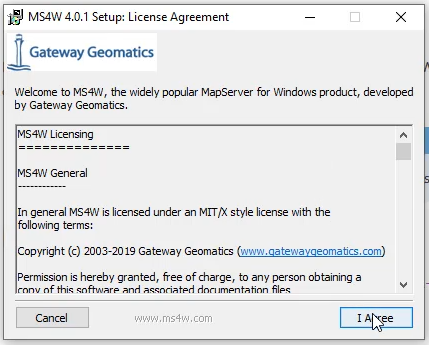
\includegraphics[width=8cm]{figures/1174006/4/3.png}
		\centering
		\caption{Klik "I Agree".}
	\end{figure}
	\item  Pilih tipe instalasinya yang "Full". Kemudian klik Next.
	\hfill\break
	\begin{figure}[H]
		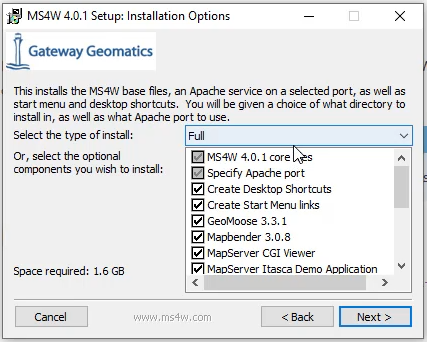
\includegraphics[width=8cm]{figures/1174006/4/4.png}
		\centering
		\caption{Tipe instalasi "Full".}
	\end{figure}
	\item  Pilih direktori instalasinya. Kemudian klik Next.
	\hfill\break
	\begin{figure}[H]
		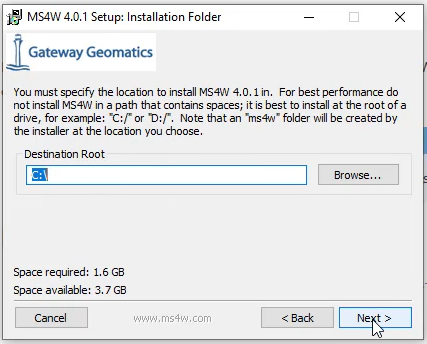
\includegraphics[width=8cm]{figures/1174006/4/5.png}
		\centering
		\caption{Pilih direktori instalasi}
	\end{figure}
	\item  Isi port Apache yang akan dipakai. Kemudian klik Next.
	\hfill\break
	\begin{figure}[H]
		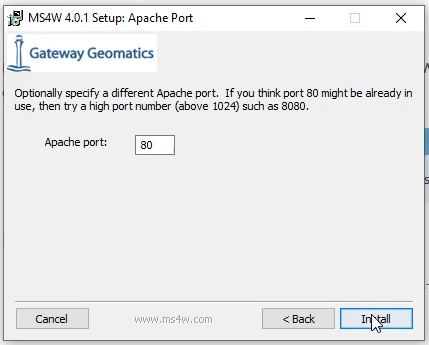
\includegraphics[width=8cm]{figures/1174006/4/6.png}
		\centering
		\caption{Isi port Apache.}
	\end{figure}
	\item  Tunggu hingga proses instalasi selesai.
	\hfill\break
	\begin{figure}[H]
		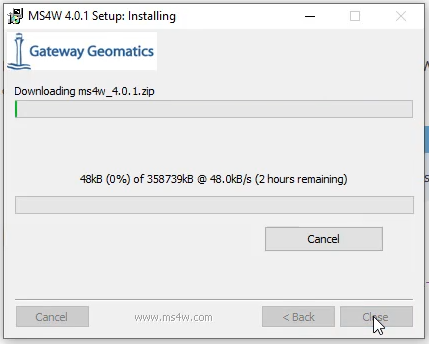
\includegraphics[width=8cm]{figures/1174006/4/7.png}
		\centering
		\caption{Proses instalasi.}
	\end{figure}
	\item  Klik Close.
	\hfill\break
	\begin{figure}[H]
		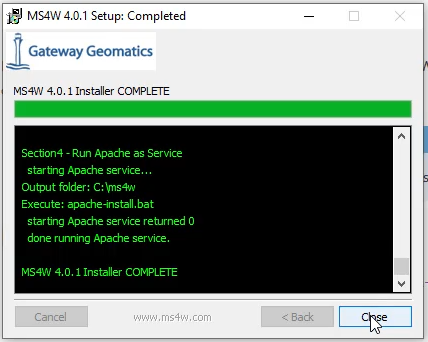
\includegraphics[width=8cm]{figures/1174006/4/8.png}
		\centering
		\caption{Akhir proses instalasi.}
	\end{figure}
\end{enumerate}
\subsection{Link Youtube}
\href{https://www.youtube.com/watch?v=g6EfXa3GtEs}{https://www.youtube.com/watch?v=g6EfXa3GtEs}
\subsection{Instalasi Map Proxy}
\begin{enumerate}
	\item  Ketik peritah berikut di CMD.
	\hfill\break
	\begin{figure}[H]
		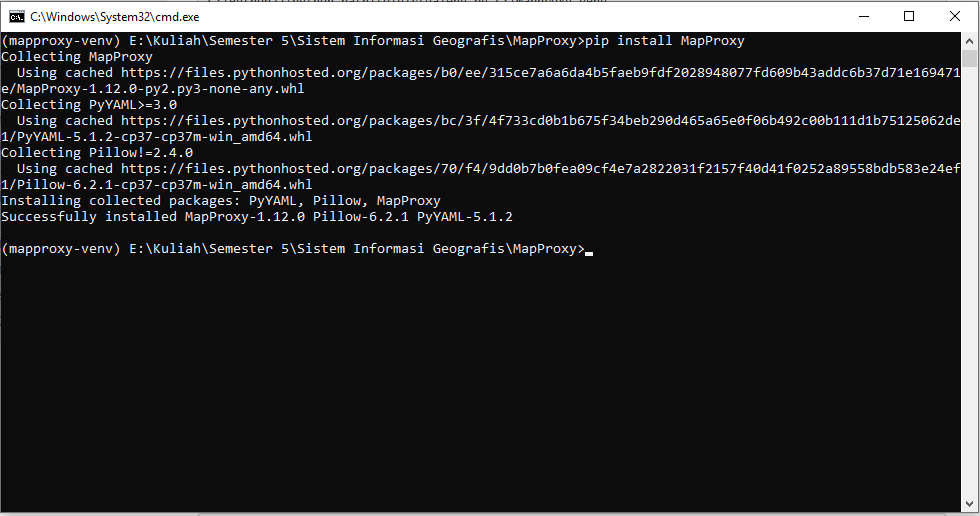
\includegraphics[width=8cm]{figures/1174006/4/11.png}
		\centering
		\caption{Install Map Proxy}
	\end{figure}
	\item  Ketik peritah berikut di CMD.
	\hfill\break
	\begin{figure}[H]
		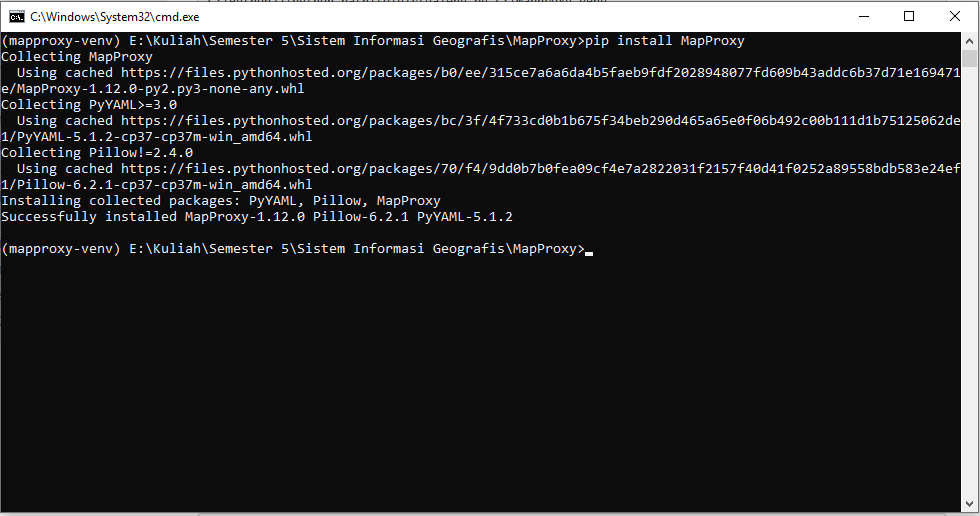
\includegraphics[width=8cm]{figures/1174006/4/11.png}
		\centering
		\caption{Install pyproj}
	\end{figure}
\end{enumerate}
\subsection{Link Youtube}
\href{https://www.youtube.com/watch?v=wJ818Tp7lzE}{https://www.youtube.com/watch?v=wJ818Tp7lzE}